\chapter{Інтерфейс МІА:СЕД}

\section{Загальний опис}

Головне меню Робочого столу користувача представлене розділами, категоріями
та активними елементами, що оптимізують роботу з документами (позначені
цифрами на Рисунку 4.1.1).

\begin{figure}[!htbp]
\centerline{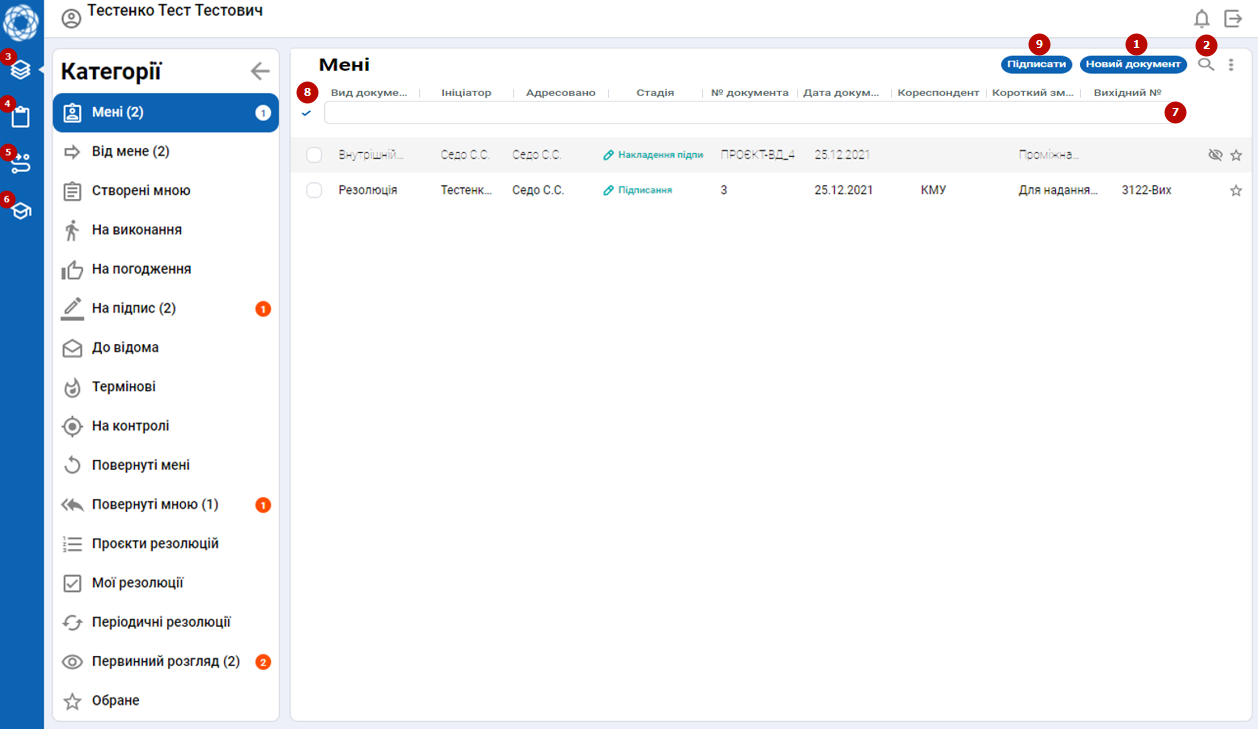
\includegraphics[width=\textwidth]{img/4.1.1.png}}
\caption{Рис. 4.1.1. Інтерфейс робочого столу користувача}
\end{figure}

Значення активних елементів Головного меню:
а) кнопка «Новий документ» (1) --- викликає появу поля для додавання
документу, на бічній панелі активізується категорія для вибору виду документа
(внутрішній/ організаційно-розпорядчий/ вихідний документ);
б) піктограма (2) --- дозволяє швидко віднайти файл/ документ серед інших за
введеними користувачем параметрами пошукового запиту (номер документа,
дата, резолюція тощо);
в) вкладка бічного меню (3) --- відкриває категорії документів;
г) вкладка бічного меню (4) --- представлена звітністю;
д) вкладка бічного меню (5) --- «Делегування прав»;
ж) вкладка бічного меню (6) --- представлена Посібником, що містить Загальні
відомості про Систему та Інструкцію користувача;
з) «Рядок фільтру» (7);
і) «Відмітка для мультипідпису» (8)
к) «Підписати» (9) --- система підписує документ.

\section{Робочий стіл користувача}

Меню Робочого столу користувача (див. Рисунок 4.2.1) представлене основними
категоріями: Мені. Від мене. Термінові. Обране.

\begin{figure}[!htbp]
\centerline{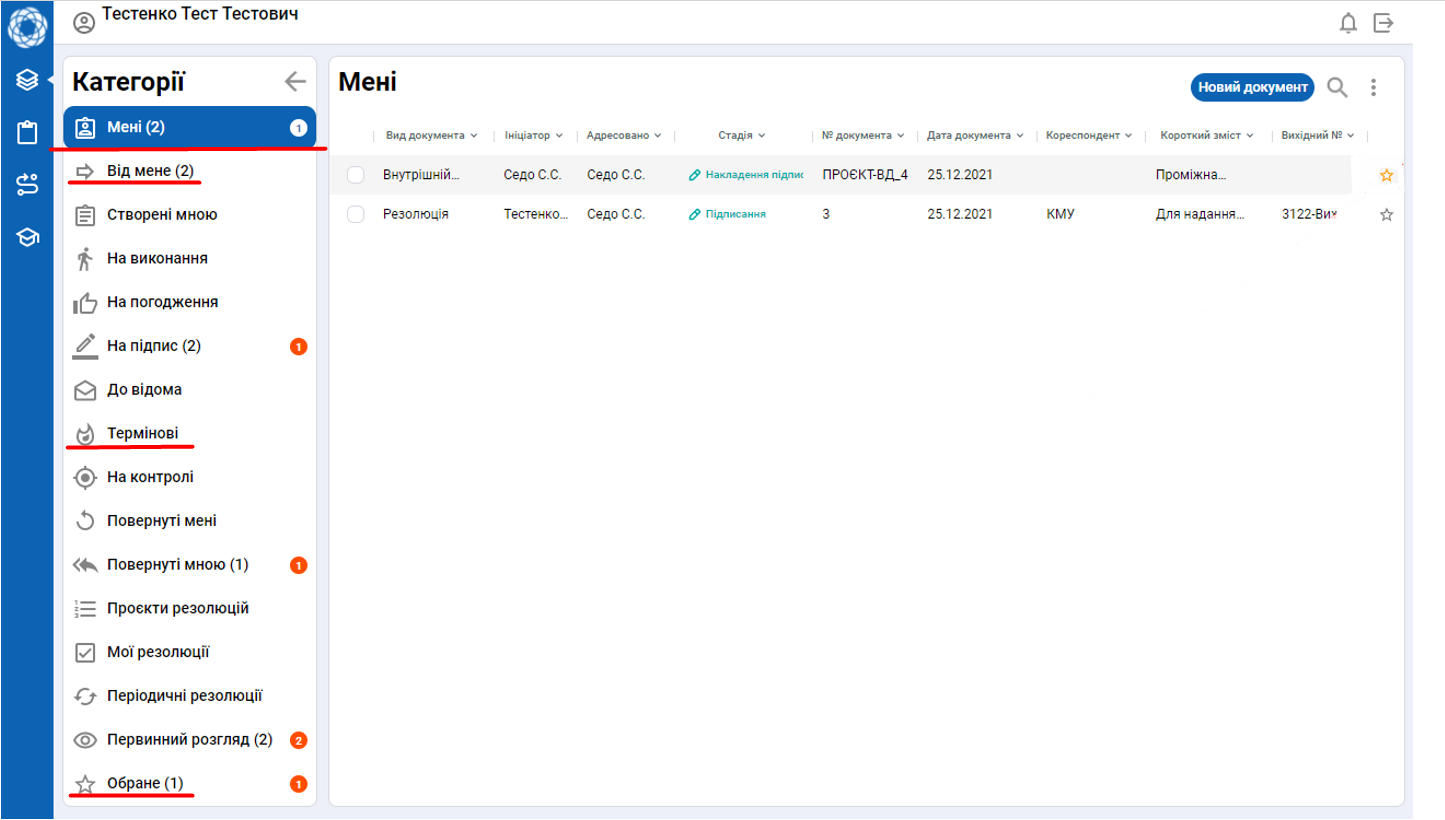
\includegraphics[width=\textwidth]{img/4.2.1.png}}
\caption{Рис. 4.2.1. Меню Робочого столу користувача}
\end{figure}

Характеристика категорій Робочого столу користувача:
 а) «Мені» --- категорія містить зведений перелік документів та задач, які
користувач має опрацювати. Документи з категорії «Мені» додатково
відображаються в інших категоріях, назви яких вказують на дії, що необхідно
здійснити з вищезгаданими документами (первинний розгляд, на підпис тощо);
 б) «Від мене» --- категорія відображає опрацьовані документи;
 в) «Термінові» --- в даній категорії відображаються службові документи зі
встановленим строком виконання (п’ять днів або менше);
 г) «Обране» --- категорія містить документи, які користувач відмітив для себе
з певних причин для швидкого доступу до них.
 Примітка: щоб відмітити документ серед переліку інших (в роботі), як обраний ---
слід натиснути на піктограму-зірочку у правому верхньому куті екранної форми Меню,
колір піктограми-зірочки змінить чорний колір на оранжевий і документ додатково
з’явиться в категорії «Обране». Повторний клік на піктограму скасує відмітку.

\section{Електронний документ в Системі}

Електронним вважається документ, інформація в якому зашифрована у вигляді
електронних даних, з можливістю створення, передачі, збереження та
перетворення електронними засобами у візуальну форму (відображення даних
документа має бути придатним для сприйняття його змісту людиною), як за
участю електронних засобів, так і у вигляді паперової форми.
В Системі виділяють вхідні, вихідні, внутрішні та організаційно-розпорядчі види
документів:
а) вхідні документи --- документи, які надійшли з інших організацій, зокрема від
юридичних осіб або громадян. До них відносяться звернення громадян, запити на
публічну інформацію тощо;
б) вихідними документами --- є документи, які адресовано за межі організації,
зокрема юридичним особам або громадянам. До них відносяться відповіді на
вхідні листи, запити, звернення тощо;
в) внутрішні документи --- документи, обіг яких здійснюється в межах організації.
До них відносяться внутрішній лист, службова, доповідна записка, доручення
тощо;
г) організаційно-розпорядчі документи --- це сукупність управлінської
документації, що представлена постановами, ухвалами, розпорядженнями,
наказами, вказівками тощо.
Усі документи в Системі рухаються певним маршрутом, стадії якого представлені
на Рисунку 4.3.1

\begin{figure}[!htbp]
\centerline{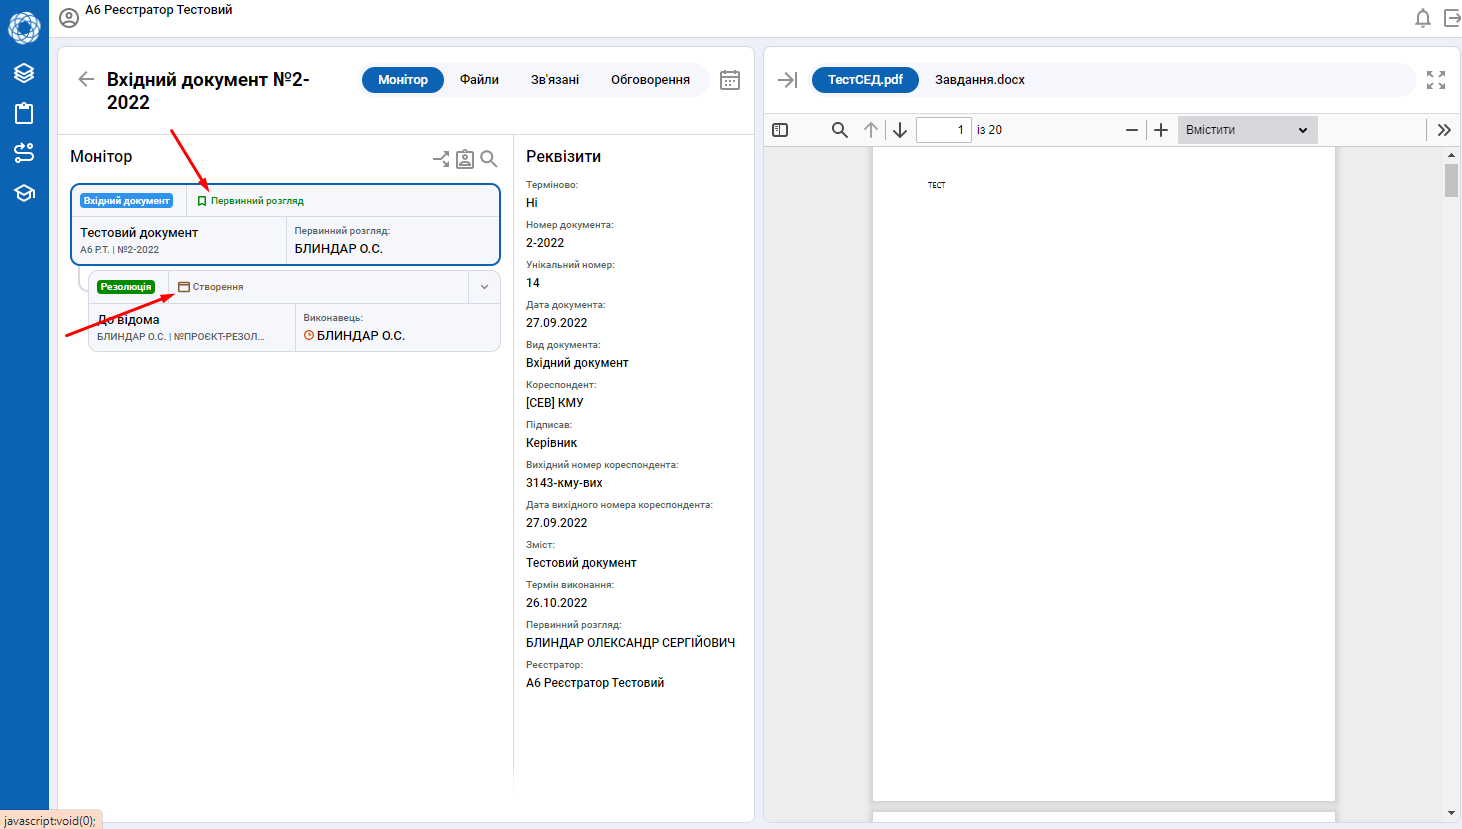
\includegraphics[width=\textwidth]{img/4.3.1.png}}
\caption{Маршрут документа в Системі}
\end{figure}

\newpage

\section{Переміщення документа в Системі}

Основними етапами документообігу в організації є:
а) обробка документів, що надходять в установу;
б) попередній розгляд документа працівниками відділу документального
забезпечення;
в) створення реєстраційно-моніторингової картки (далі РМК);
г) організація раціонального руху документа в Системі:
1) доведення документа до виконавця;
2) контроль за виконанням;
3) проходження, узгодження та підпис проєктів документів;
4) обробка виконаних документів та їх відправка.
Маршрут документа в Системі:
− «Реєстрація» характерна для вхідних документів. Відповідальними
особами на стадії реєстрації, обліку та організації документообігу є
працівники відділу документального забезпечення, які:
1) здійснюють експедиційне опрацювання, результатом якого є створення
реєстраційно-моніторингової картки (далі РМК) до якої вносяться всі
обов’язкові, додаткові та інші облікові дані документа;
16
2) здійснюють обробку вхідної кореспонденції --- документ у паперовому
вигляді сканується та завантажується у Систему, якщо документ надходить
через Систему електронної взаємодії (далі СЕВ) або Email --- перевіряють чи
не порушено вимоги щодо форми документа, чи заявлений склад документа
відповідає фактичному, чи збігаються реквізити, наявність пов’язаного з
електронним документом кваліфікованого електронного підпису тощо;
3) на даному етапі є можливість змінювати РМК, додавати документ і додатки,
видаляти основний документ і додатки, створювати проєкти резолюцій,
визначати особу первинного розгляду.

\begin{figure}[!htbp]
\centerline{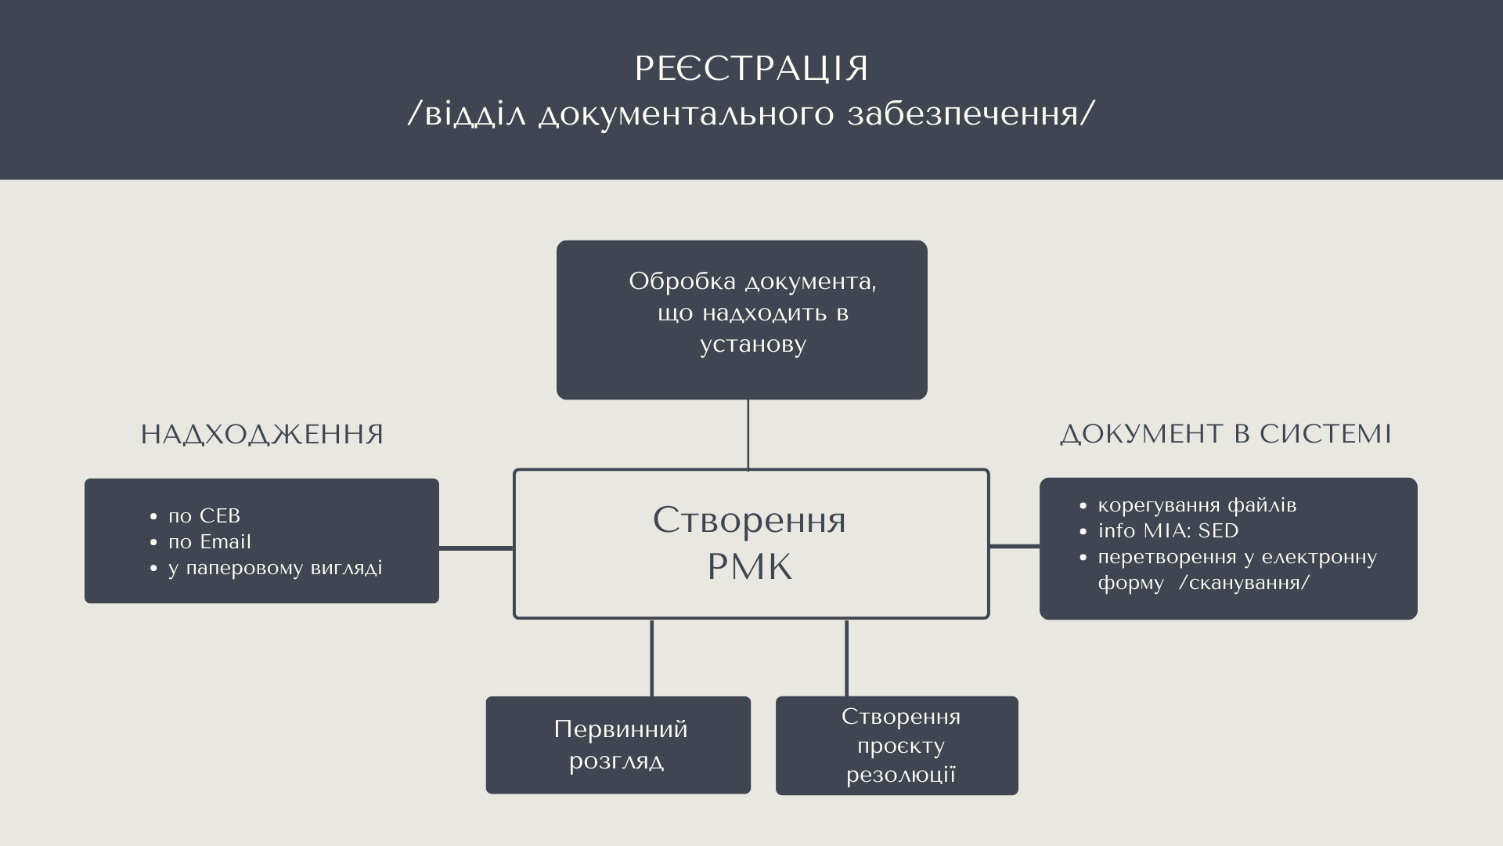
\includegraphics[width=\textwidth]{img/4.4.1.png}}
\caption{Рис. 4.4.1. Маршрут документа в Системі}
\end{figure}

--- «Первинний розгляд» після реєстрації документ надходить на первинний
розгляд відповідальним особам, згідно розподілу функціональних
обов’язків (помічник директора) для створення резолюції. Створюється
маршрут розгляду документа, прямує до керівника на визначення.

\begin{figure}[!htbp]
\centerline{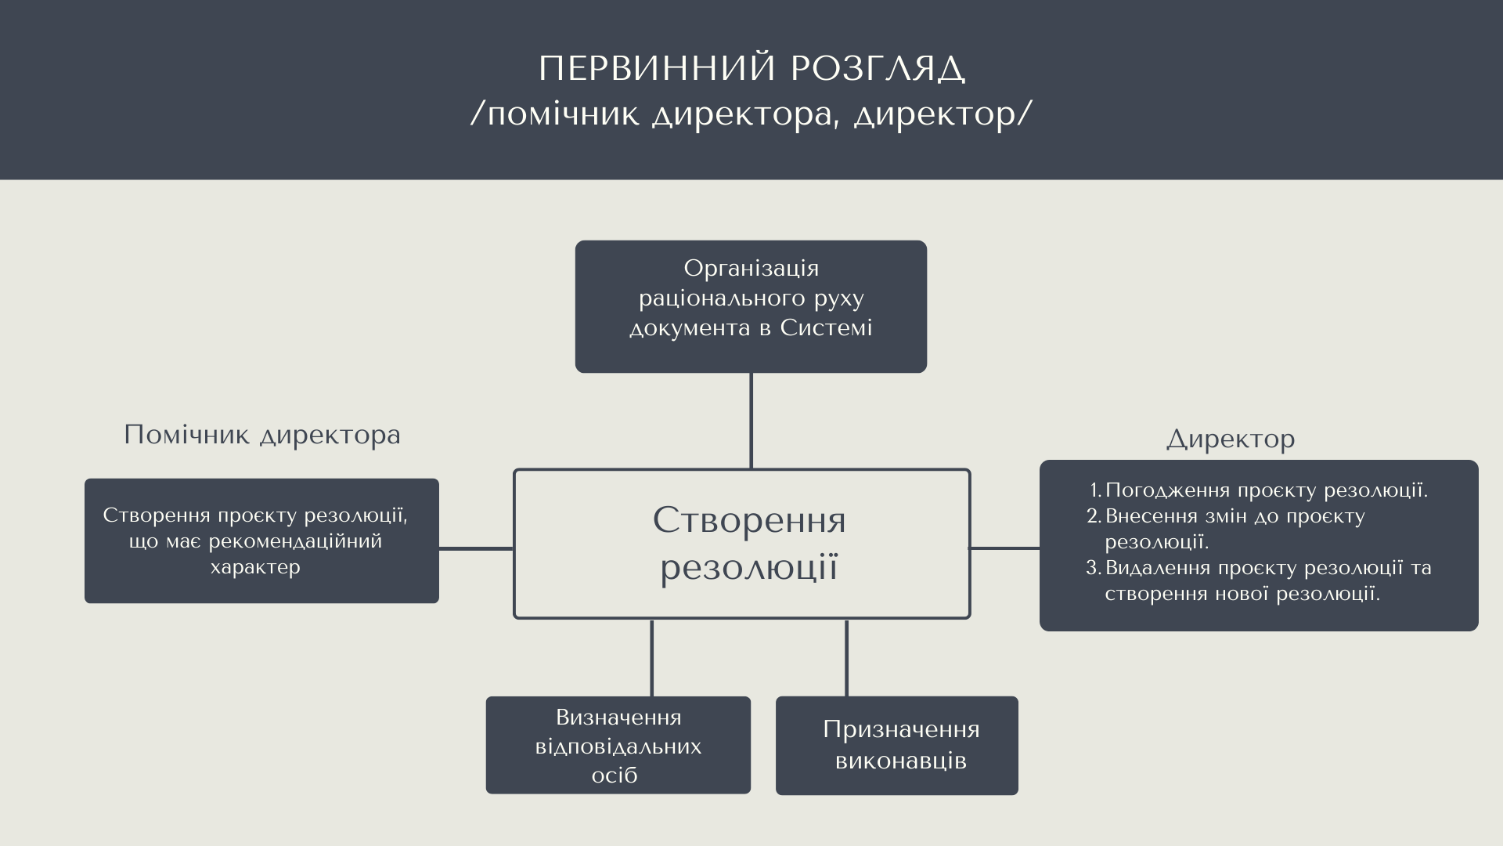
\includegraphics[width=\textwidth]{img/4.4.2.png}}
\caption{Рис. 4.4.2. Схематичне зображення етапу Первинний розгляд. Створення резолюції}
\end{figure}

--- «Створення резолюції» посадова особа, що здійснює первинний розгляд
електронного документа, накладає на нього електронну резолюцію, в якій
визначає головного виконавця, відповідального за перелік задач, що
необхідно виконати по даному документу, та, у разі необхідності,
співвиконавців і строк його виконання.
--- «Виконання» виконавці здійснюють роботу над документом з можливістю
розпису резолюцій на підлеглих (вторинна резолюція), створення проєктів
документів.
--- «Розробка проєкта» Власник стадії – користувач, який є автором проєкта
документа. На стадії «Розробка проєкта» автор може вносити зміни в РМК,
редагувати основний документ, додавати додатки, виправляти додатки,
видаляти основний документ і додатки, формувати список погодження,
направляти проєкт документа на погодження.

\begin{figure}[!htbp]
\centerline{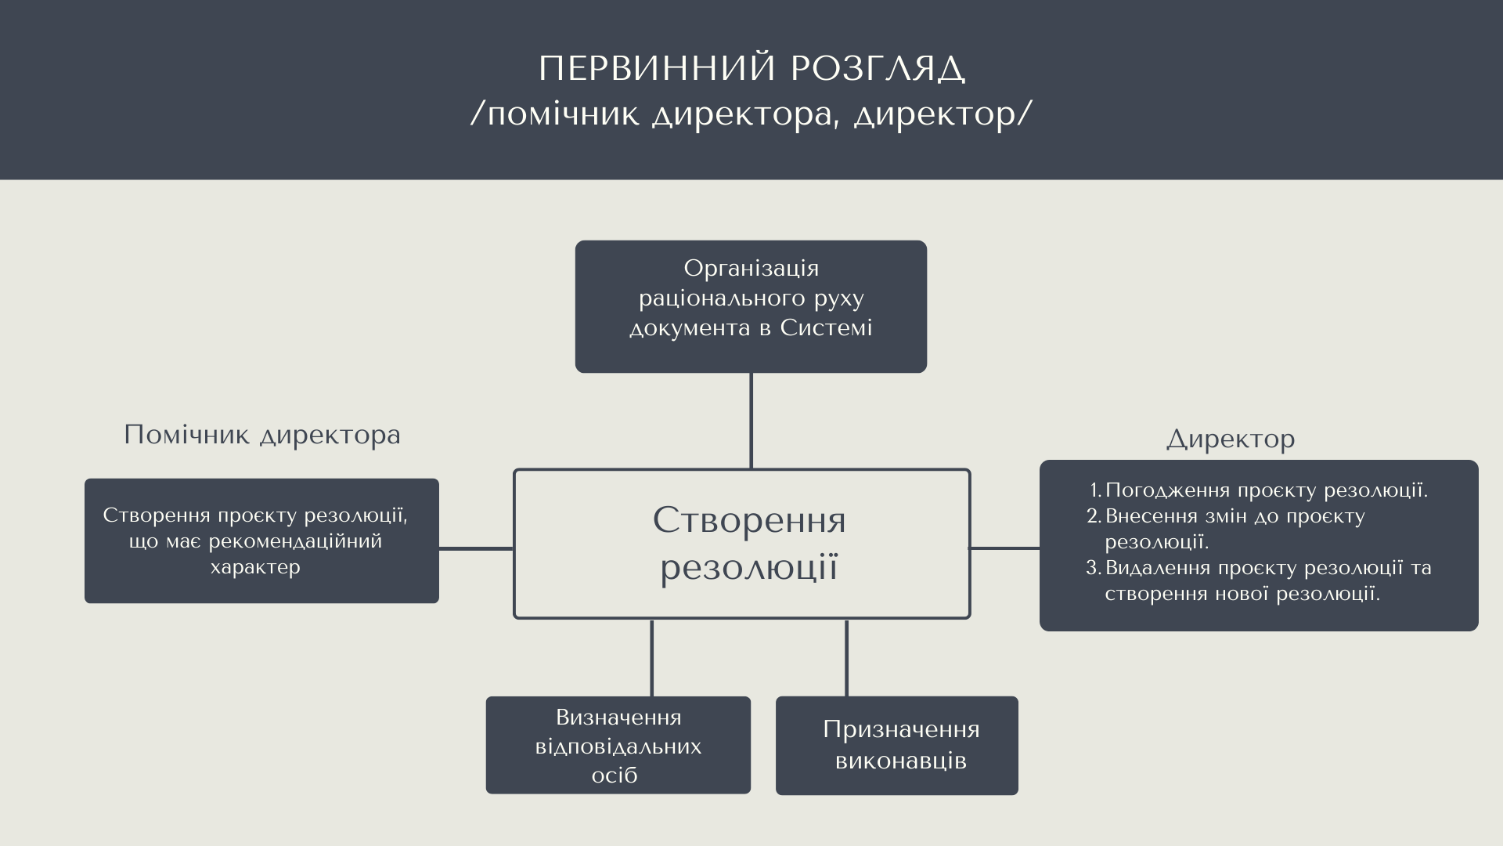
\includegraphics[width=\textwidth]{img/4.4.2.png}}
\caption{Рис. 4.4.2. Схематичне зображення етапу Виконання}
\end{figure}

--- «Погодження» призначена для автоматизації процесів узгодження,
ознайомлення, перевірки, розгляду, візування. На даному етапі можна:
1) визначати і додавати до листа погодження нових погоджувачів;
2) погоджувачі проєкту документа мають можливість повернути його
на стадію розробки проєкта;
3) повернути на доопрацювання попередньому погоджувачу;
4) погодити документ.
--- «Накладення підпису» присутня у внутрішніх та вихідних документах. Після
«Погодження» проєкт документа потрапляє до підписувача на стадію
«Підпис», який може підписати запропонований йому проєкт документа,
повернути проєкт документа на стадію «Розробка проєкта» або створити
власну версію проєкта документа та підписати його. Налаштована функція
попереднього перегляду документа відповідальною особою (помічник
директора) для перевірки дотримання вимог оформлення вихідного
документа і, за необхідності – повернути документ на стадію розробки
проєкту. Після підписання документ прямує на відправку.

\begin{figure}[!htbp]
\centerline{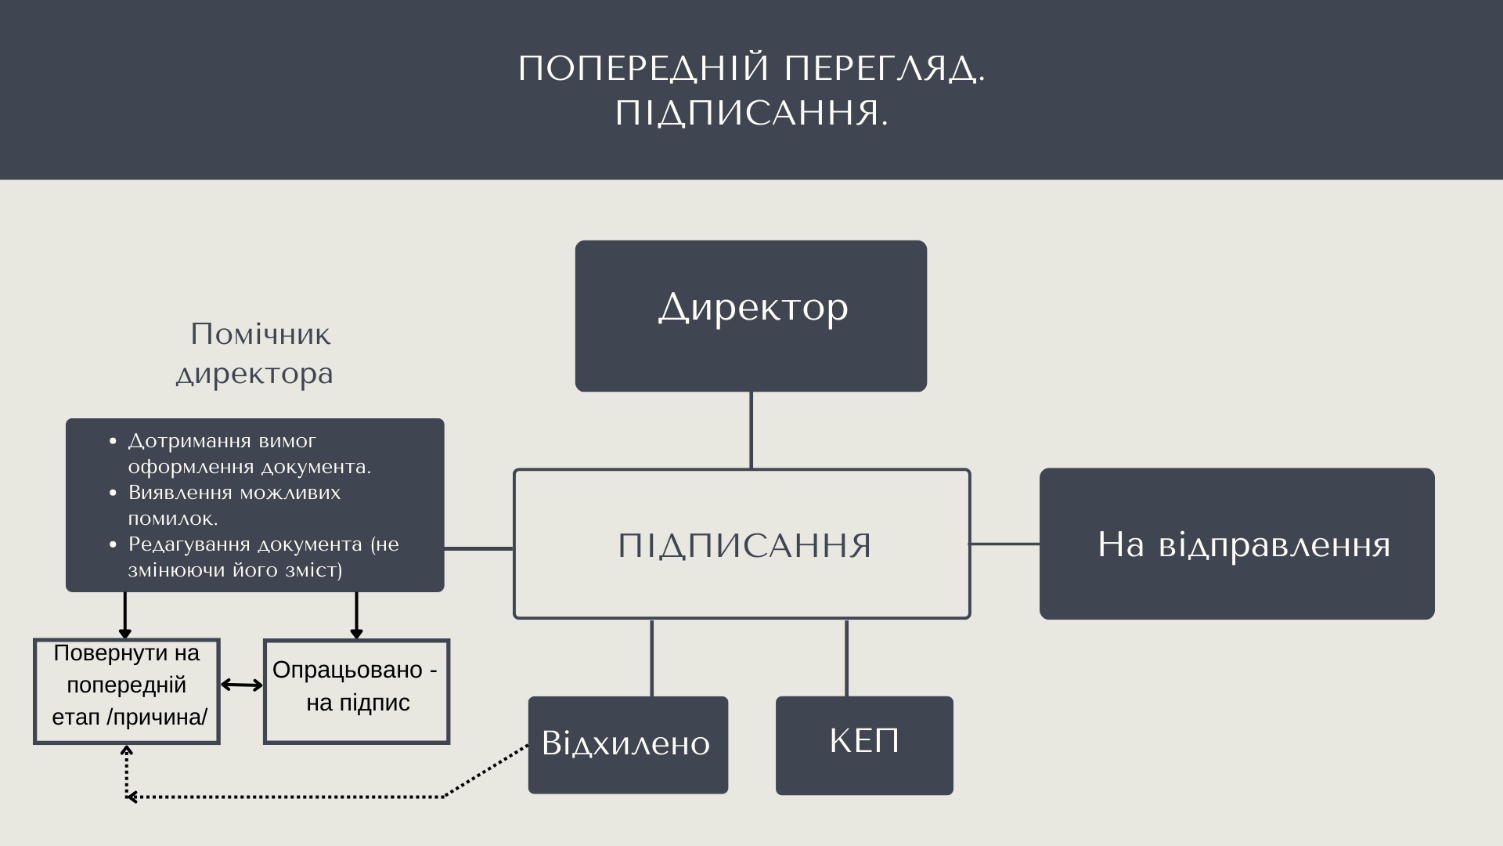
\includegraphics[width=\textwidth]{img/4.4.4.png}}
\caption{Рис. 4.4.4. Схематичне зображення етапу Накладення підпису}
\end{figure}

--- «Відправка документа» вихідні документи перед відправкою інспектуються
працівниками відділу документального забезпечення (реєстраторами) для
перевірки правильності вибору способу відправки/ доставки. Види
відправлення документів до адресата:
1) по СЕВ із СЕД;
2) по Email із СЕД;
3) кореспонденція в паперовій формі (лист з повідомленням, нарочно,
доставка кур’єром).
--- «Групування» - етап присутній в усіх документах де були розписані та
виконані усі резолюції по документу. На даному етапі реєстратори мать
можливість внести зміни до номенклатури документа.
--- Документ переміщується до архіву на «Зберігання» - ознака, що документ
опрацьований з дотриманням вимог оформлення документів. Документи
доступні тільки для перегляду.

\section{Інтерфейс документа}

Візуальний вигляд документа (проєкт документа) представлено на Рисунку 4.5.1

\begin{figure}[!htbp]
\centerline{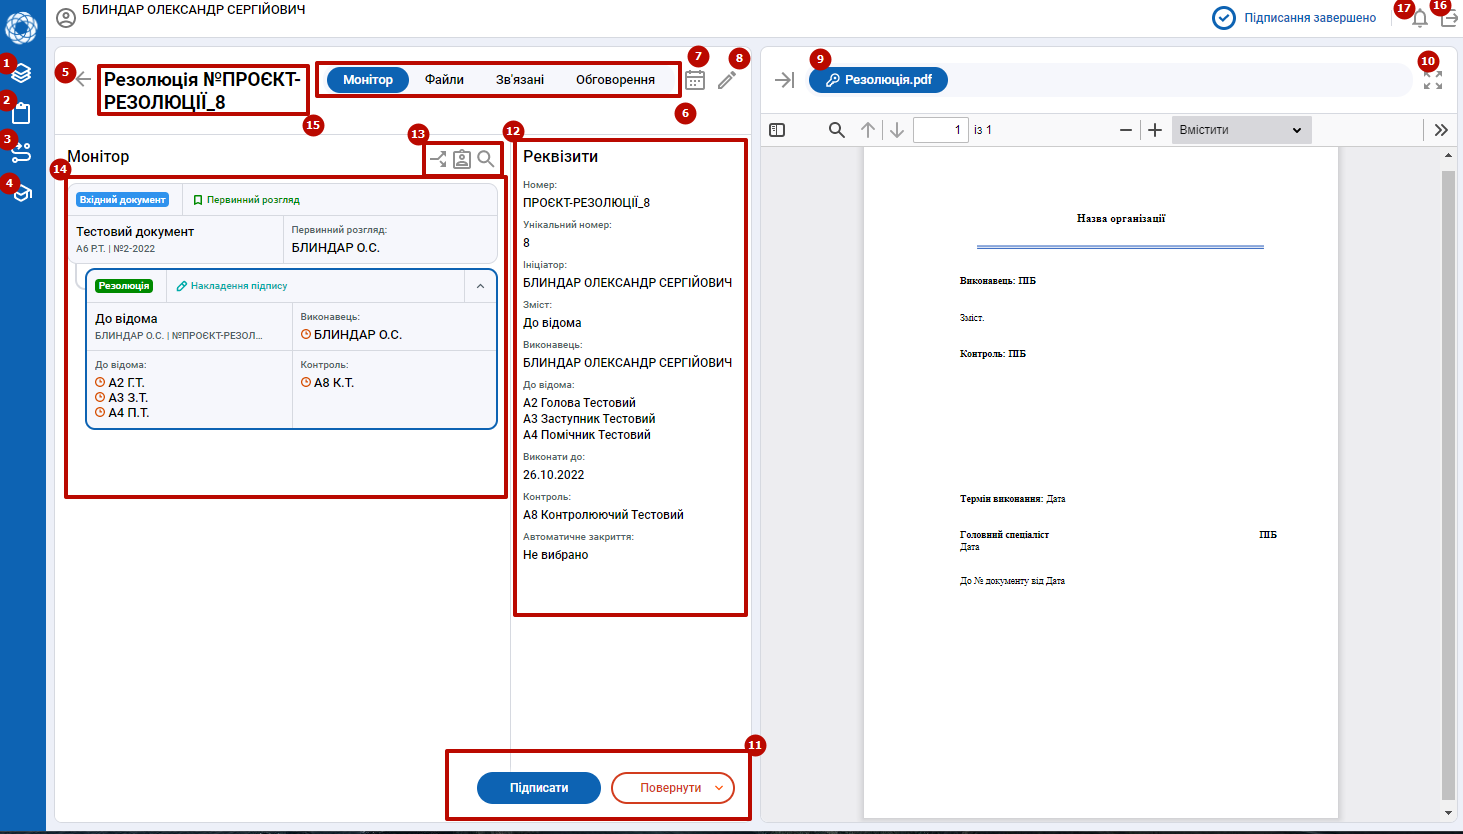
\includegraphics[width=\textwidth]{img/4.5.1.png}}
\caption{Рис. 4.5.1. Візуальний вигляд проєкту документа}
\end{figure}

Значення активних елементів, що позначені цифрами на Рисунку 4.5.1:

\circled{1} --- категорії документів;
\circled{2} --- звітність;
\circled{3} --- делегування прав;
\circled{4} --- посібник (загальні відомості про систему, інструкція користувача);
\circled{5} --- кнопка «Назад» - повернення на попередній рівень;
\circled{6} --- вкладки по обраному процесу;
\circled{7} --- історія по обраному процесу;
\circled{8} --- редагування (спільна кнопка для внесення змін у проєкт документа (проєкт резолюції, реквізити вхідного документа);
\circled{9} --- основний файл (той що з позначкою «ключ»);
\mymk{10} --- розгорнути на весь екран поточний файл;
\mymk{11} --- кнопки відпрацювання обраного процесу (в залежності від процесу кнопки можуть змінюватись, але розташування залишається незмінним);
\mymk{12} --- реквізити обраного процесу (можуть бути як реквізити проєкта документа, так і резолюції);
\mymk{13} --- навігація по монітору;
\mymk{14} --- монітор --- відображення списку всіх процесів;
\mymk{15} --- назва та номер основного документа;
\mymk{16} --- кнопка виходу із облікового запису;
\mymk{17} --- кнопка сповіщення.

Окремі активні елементи містять в своєму складі підпорядковані додаткові
можливості. Опис їх функціоналу представлений нижче.

\begin{figure}[!htbp]
\centerline{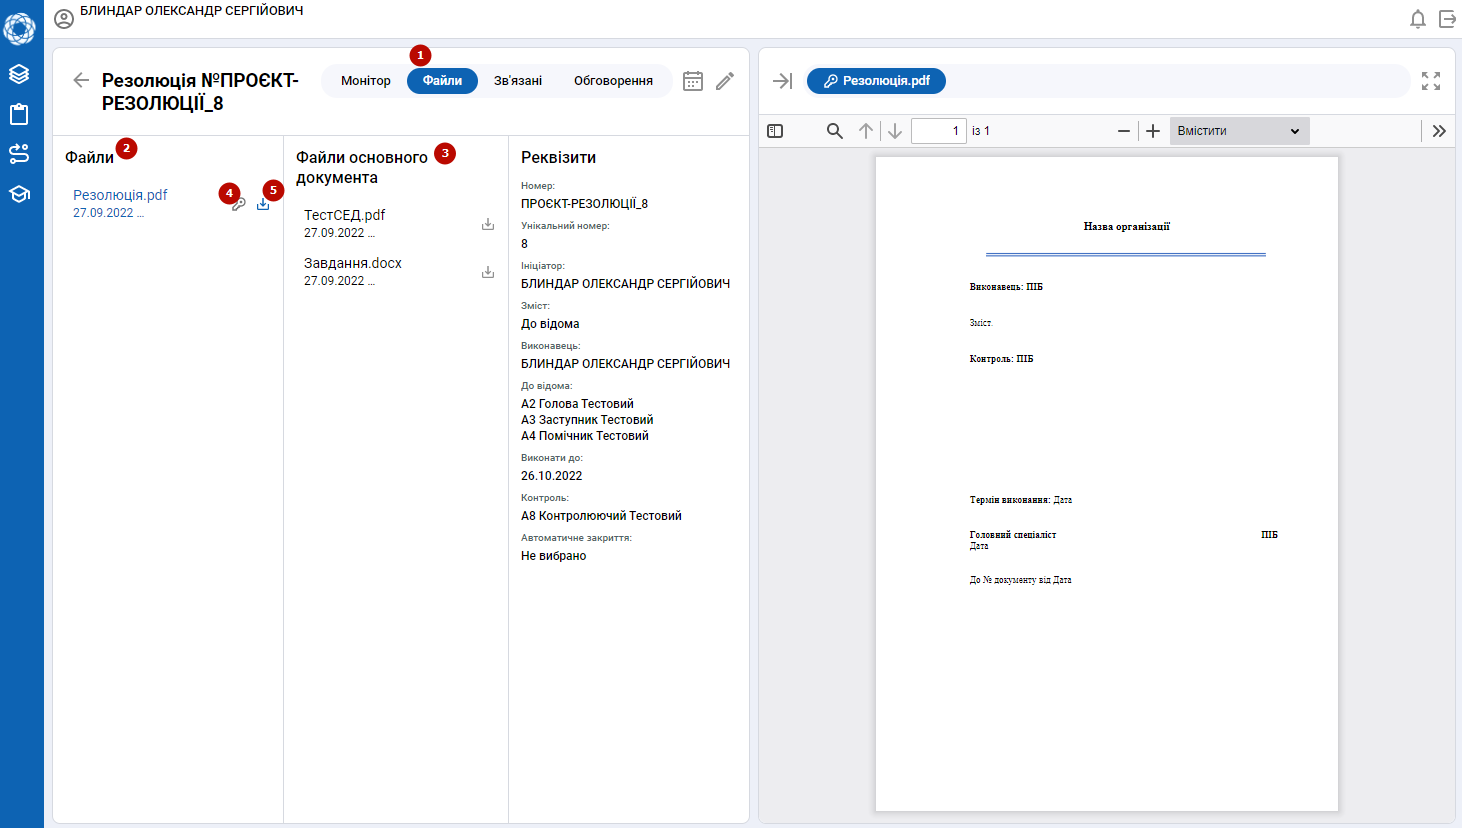
\includegraphics[width=\textwidth]{img/4.5.2.png}}
\caption{Рис. 4.5.2. Bкладка Файли}
\end{figure}

Цифрами на Рисунку 4.5.2 позначено:

\circled{1} --- кнопка виклику всіх файлів;
\circled{2} --- список файлів;
\circled{3} --- файли основного документа;
\circled{4} --- підпис (КЕП);
\circled{5} --- функція завантаження поточного файлу.

Функціонал вкладки по обраному процесу Зв’язані документи представлений на
Рисунку 4.5.3.

\begin{figure}[!htbp]
\centerline{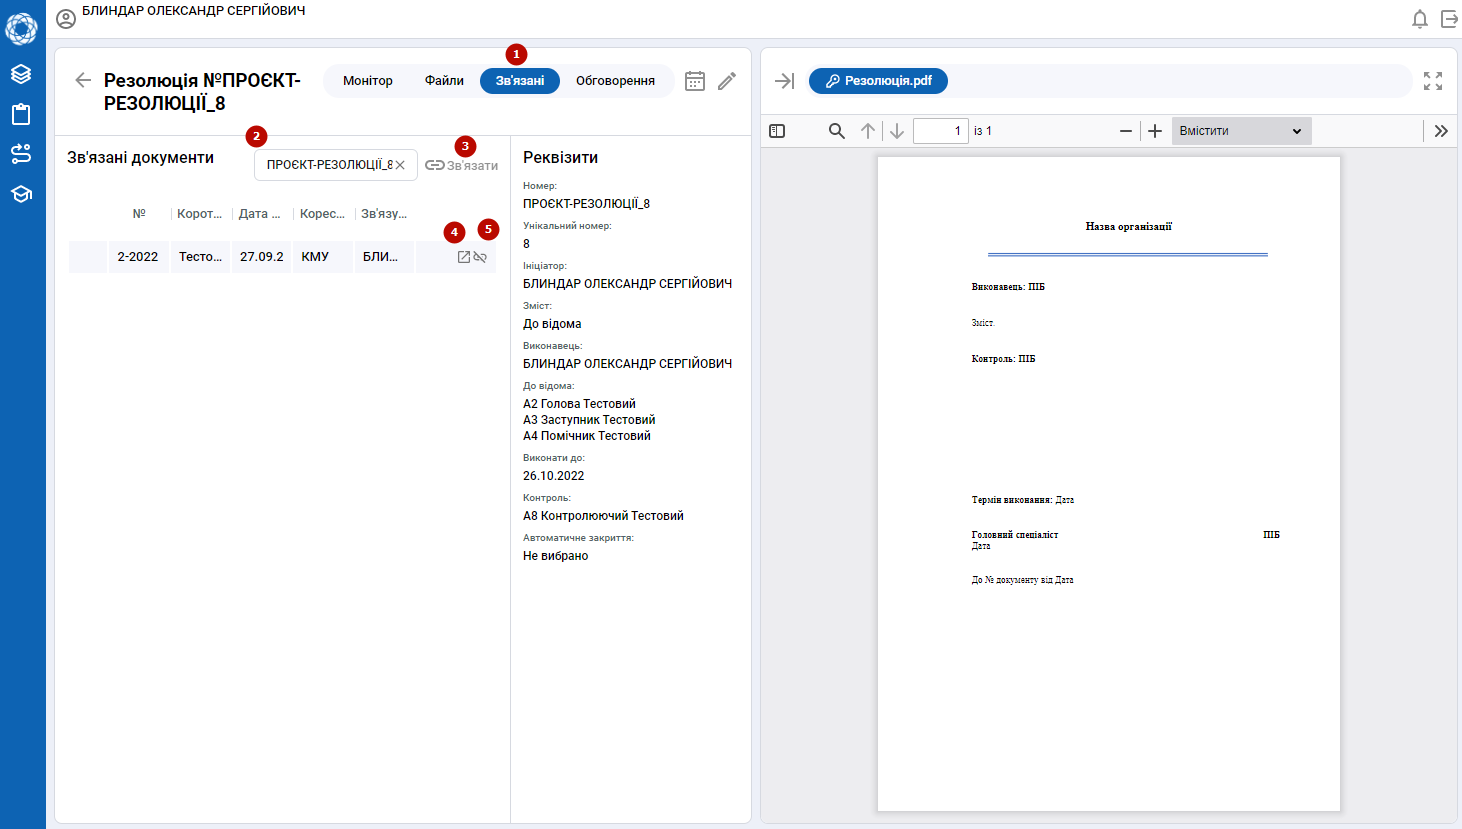
\includegraphics[width=\textwidth]{img/4.5.3.png}}
\caption{Рис. 4.5.3. Bкладка Зв'язані документи}
\end{figure}

Цифрами на Рисунку 4.5.3 позначено:

\circled{1} --- поточна вкладка;
\circled{2} --- вибір процесу зв’язування (за замовчуванням --- поточний);
\circled{3} --- кнопка «Зв’язати»;
\circled{4} --- кнопка «Перейти у документ»;
\circled{5} --- кнопка «Відв’язати».

Функціонал вкладки по обраному процесу Обговорення представлений на
Рисунку 4.5.4.

\begin{figure}[!htbp]
\centerline{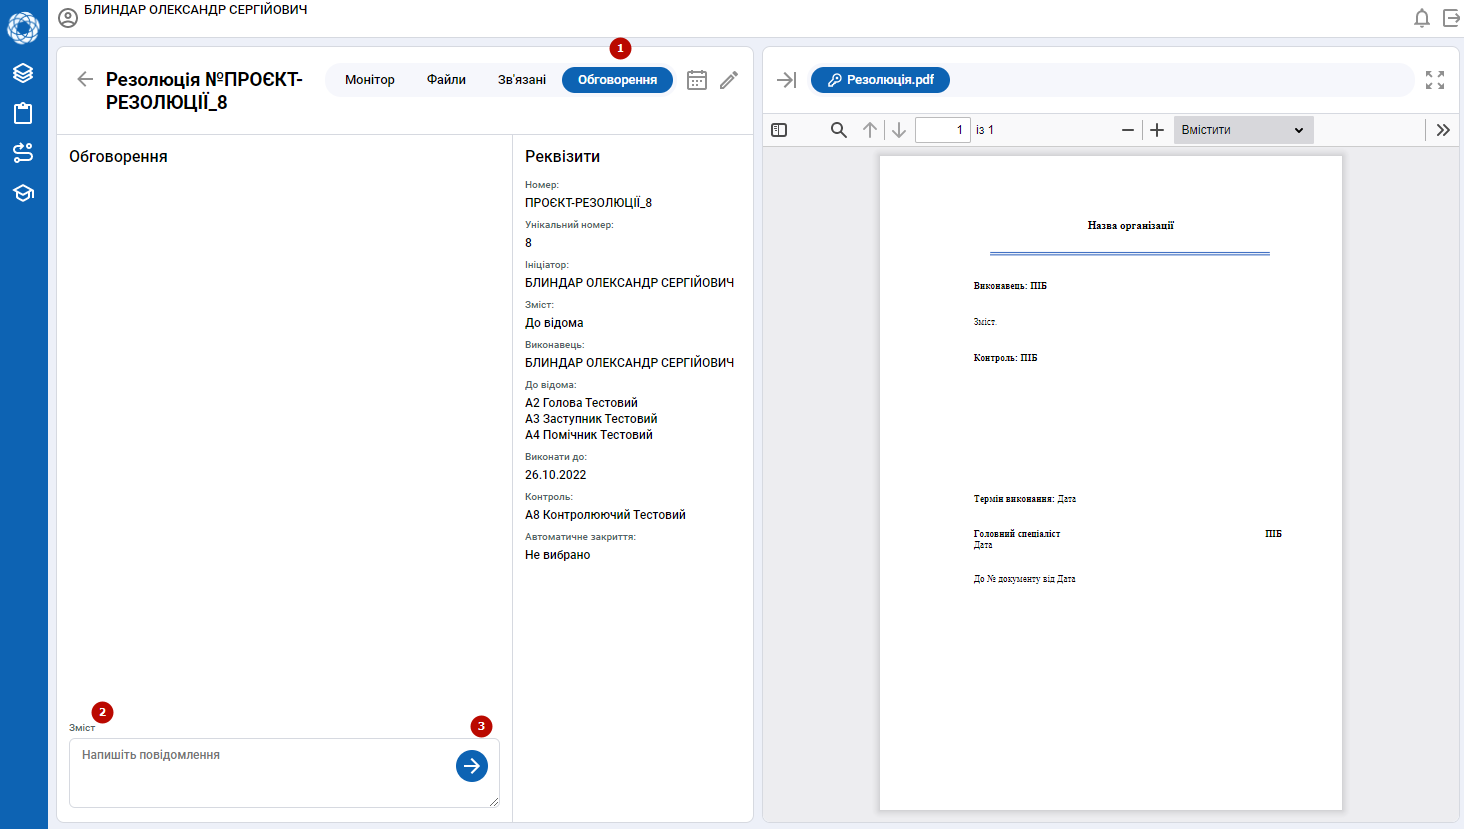
\includegraphics[width=\textwidth]{img/4.5.4.png}}
\caption{Рис. 4.5.4. Bкладка Обговорення}
\end{figure}

Цифрами на Рисунку 4.5.4 позначено:
\circled{1} --- поточна вкладка;
\circled{2} --- область для введення повідомлення;
\circled{3} --- кнопка надсилання повідомлення.

Функціонал вкладки Історія по обраному процесу (розгорнуте підменю
піктограми 7 див. Рисунок 4.5.1).

\begin{figure}[!htbp]
\centerline{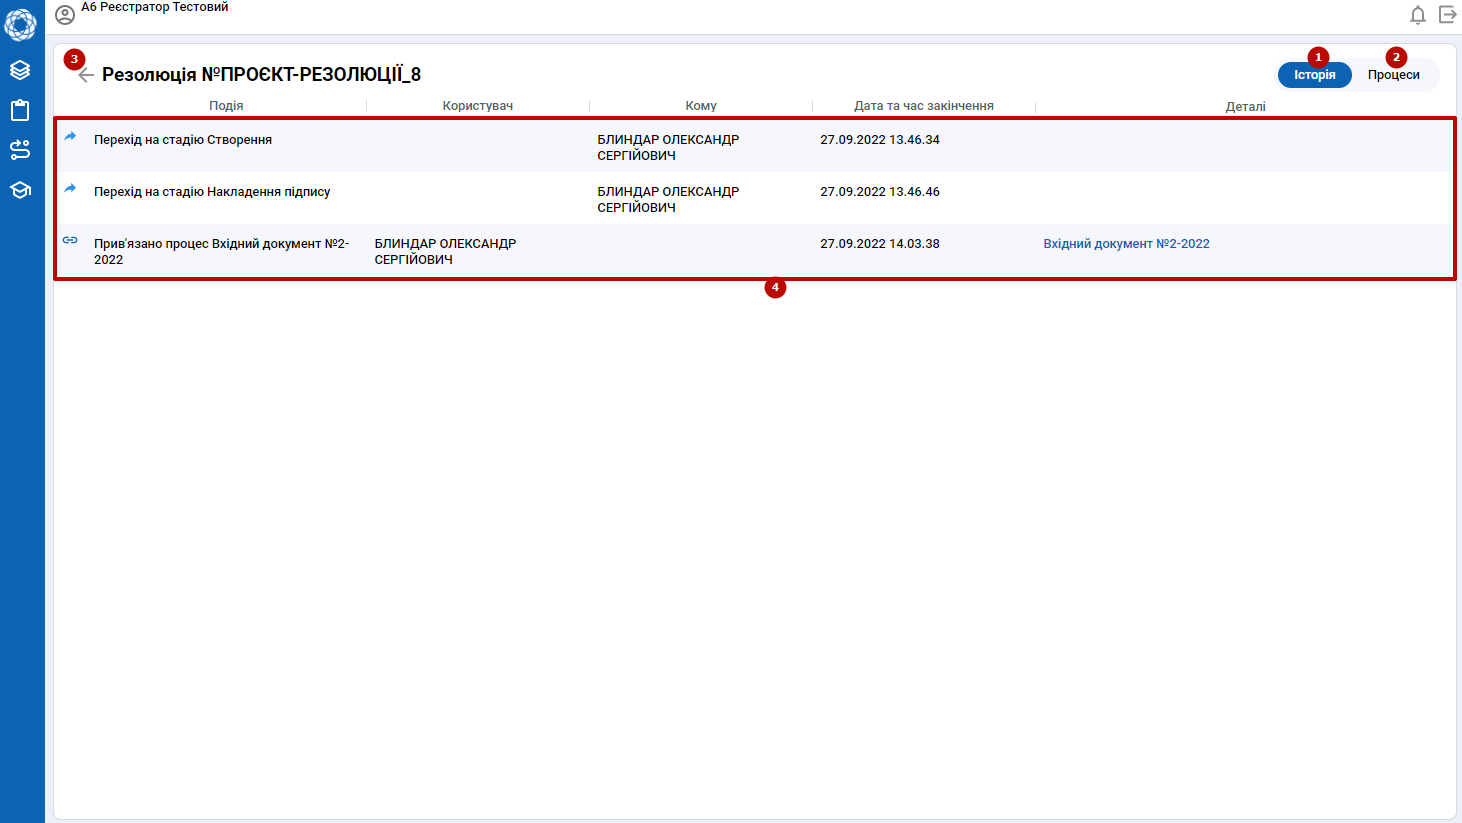
\includegraphics[width=\textwidth]{img/4.5.5.png}}
\caption{Рис. 4.5.5. Історія по обраному процесу}
\end{figure}

Цифрами на Рисунку 4.5.5 позначено:

\circled{1} --- поточна вкладка Історія;
\circled{2} --- кнопка переходу на відображення схеми бізнес-процесу (див. Рисунок 4.5.6);
\circled{3} --- кнопка повернення до документа;
\circled{4} --- область відображення історії документа.

\begin{figure}[!htbp]
\centerline{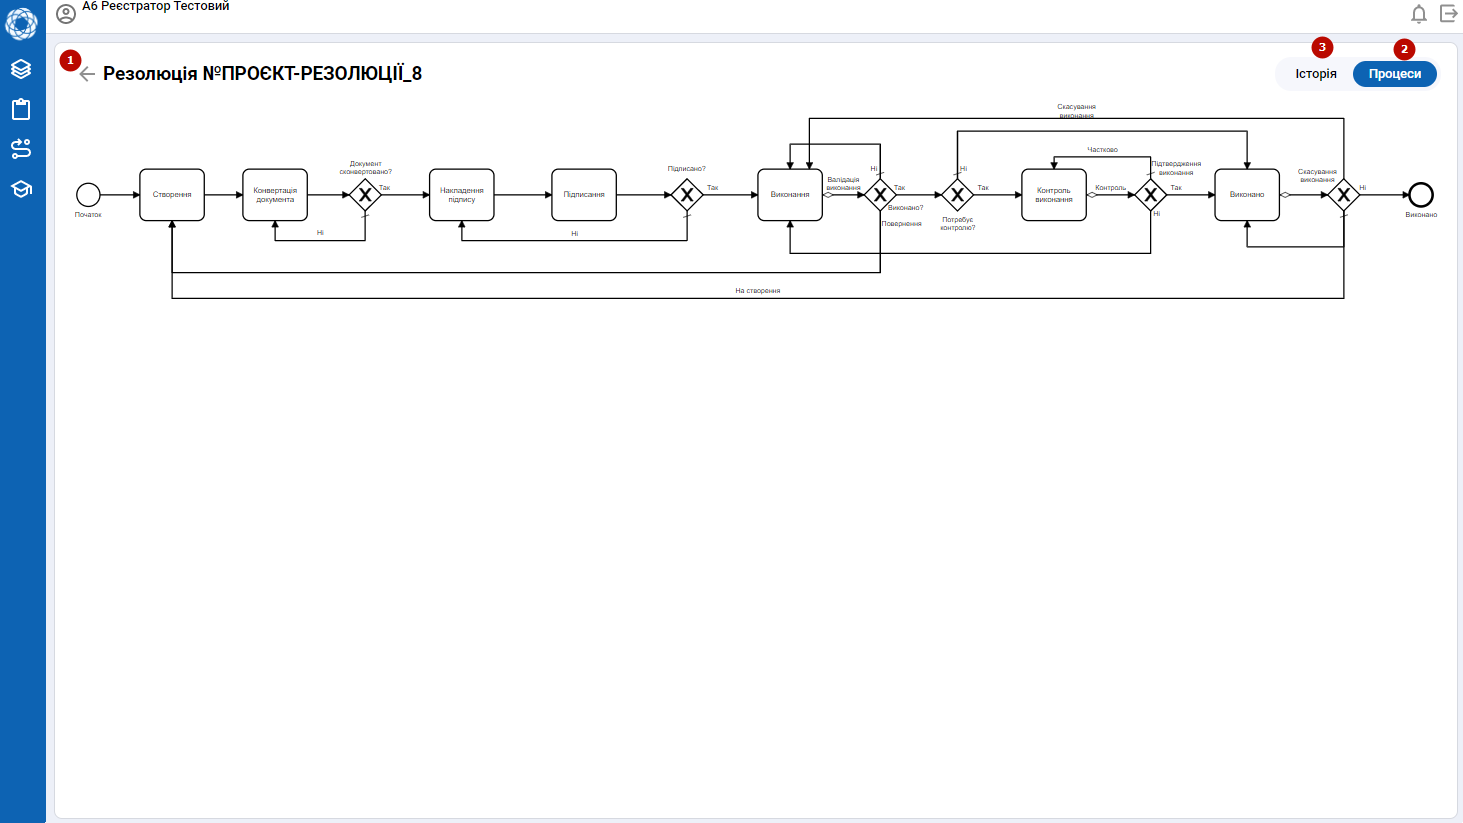
\includegraphics[width=\textwidth]{img/4.5.6.png}}
\caption{Рис. 4.5.6. Схема бізнес-процесу}
\end{figure}

Розгорнуте підменю вкладки 2 Процеси (див. Рисунок 4.5.5) позначено цифрами на Рисунку 4.5.6:

\circled{1} --- кнопка повернення документа;
\circled{2} --- поточна вкладка;
\circled{3} --- кнопка переходу на відображення історії документа.

